\documentclass[11pt]{article}
% Кодировка и язык
\usepackage[utf8]{inputenc}           % Кодировка исходного файла (UTF-8)
\usepackage[T2A]{fontenc}             % Кодировка шрифтов для кириллицы
\usepackage[english,russian]{babel}   % Локализация: русские названия, переносы

% Поиск в PDF
\usepackage{cmap}                     

% Поля страницы
\usepackage{geometry}
\geometry{left=2cm, right=2cm, top=2cm, bottom=2cm}

% Математика
\usepackage{amsmath, amssymb, amsthm} % Базовые пакеты для математики
\usepackage{mathtools}                % Расширение amsmath (доп. символы и окружения)

% Картинки
\usepackage{graphicx}                 % Вставка картинок (\includegraphics)
\graphicspath{{pictures/}}            % Путь к папке с картинками
\usepackage{float}                    % Позволяет использовать [H] для жёсткого позиционирования
\usepackage{wrapfig}                  % Обтекание текста вокруг картинок

% Таблицы
\usepackage{array}                    % Расширенные возможности для таблиц
\usepackage{booktabs}                 % Красивые таблицы (\toprule, \midrule, \bottomrule)
\usepackage{multirow}                 % Объединение строк в таблицах
\usepackage{tabularx}                 % Таблицы с автоматической шириной колонок
\usepackage{ragged2e}                 % Улучшенное выравнивание (используется в tabularx)

% Списки
\usepackage{enumitem}                 % Гибкая настройка списков (itemize, enumerate)

% Колонтитулы
\usepackage{fancyhdr}                 

% Гиперссылки
\usepackage{xcolor}                   % Работа с цветами
\usepackage{hyperref}                 % Гиперссылки, оглавление, перекрёстные ссылки

% Умные ссылки
\usepackage{cleveref}                 

% Типографика
\usepackage{microtype}                % Улучшает переносы и межсловные расстояния

% Подписи к картинкам и таблицам
\usepackage{caption}                  % Настройка подписей (шрифт, отступы)

% Рисование схем и графиков
\usepackage{tikz}                     % Рисование схем, графиков, диаграмм
\usepackage{pgfplots}                 % Построение графиков функций (на основе tikz)
\pgfplotsset{compat=newest}           % Версия совместимости pgfplots

% Алгоритмы и код
\usepackage{algorithm}                % Окружения для алгоритмов
\usepackage{algorithmic}              % Синтаксис для алгоритмов
\usepackage{listings}                 % Вставка кода с подсветкой синтаксиса


% Настройка нумерации секций и подсекций
\renewcommand{\thesection}{\arabic{section}}                   
\renewcommand{\thesubsection}{\thesection.\arabic{subsection}} 


% Настройка списков: убираем лишние отступы слева
\setlist[itemize]{leftmargin=}
\setlist[enumerate]{leftmargin=}


% Определение окружений для теорем, лемм, определений и т.д.
% Нумерация привязана к номеру секции
\newtheorem{theorem}{Теорема}[section]
\newtheorem{definition}{Определение}[section]
\newtheorem{remark}{Замечание}[section]
\newtheorem{lemma}{Лемма}[section]
\newtheorem{example}{Пример}[section]
\newtheorem{consequence}{Следствие}[section]
\newtheorem{algorithmm}{Алгоритм}
\newtheorem{question}{Вопрос}[section]
\newtheorem{answer}{Ответ}[section]
\newtheorem{statement}{Утверждение}[section]


% Определение цветов
\definecolor{pblue}{rgb}{0.13,0.13,1}    
\definecolor{pgreen}{rgb}{0,0.5,0}       
\definecolor{pred}{rgb}{0.9,0,0}         
\definecolor{pgrey}{rgb}{0.46,0.45,0.48}
\usepackage{dsfont}
\usepackage{ulem}

\DeclareMathOperator{\Cov}{cov} 

\newcommand{\lectureNumber}{7}
\newcommand{\lectureTitle}{Ковариация СВ. Дисперсия суммы многих СВ. Математическое ожидание функции от пары СВ. Коэффициент корреляции. Независимость многих СВ}
\newcommand{\courseName}{Теория вероятностей}
\newcommand{\semester}{3 семестр, 2026/2027 уч. год}

\pagestyle{fancy}
\fancyhf{}
\fancyhead[L]{Я почему вредный был? Потому что у меня \sout{велосипеда} ковариации не было}
\fancyhead[R]{\thepage}
\setlength{\headheight}{15pt}

\hypersetup{
    colorlinks=true,
    linkcolor=blue!70!black,
    citecolor=blue!70!black,
    filecolor=blue!70!black,
    urlcolor=blue!70!black,
}

\begin{document}


\begin{titlepage}
    \centering
    
    {\large Московский физико-технический институт \par}
    {\large Высшая школа программной инженерии \par}
    \vspace{2cm}

    {\Large \textbf{\courseName} \par}
    {\large \semester \par}
    
    \vspace*{\fill}

    {\Huge \textbf{Лекция \lectureNumber} \par}
    {\Huge \textbf{\lectureTitle} \par}
    
    \vspace*{\fill}
    
    {\large Лектор: Широков М.Е. <3\par}
    {\large Автор: \href{t.me/sol_m_07}{Соля} \par}

\end{titlepage}

\pagenumbering{arabic}

\section{Дисперсия бернуллиевской случайной величины}

C прошлой лекции нам известно, что для попарно независимых случайных величин $\{\xi_1, \ldots, \xi_n\}$
\[D\left(\sum_{i = 1}^{n} \xi_i\right) = \sum_{i = 1}^{n} D(\xi_i)\]
Посчитаем тогда дисперсию бернуллиевской случайной величины $\beta_n^p$. Как и при подсчёте 
математического ожидания, введём индикаторы:
\[\mathds{1}_i \text{ --- индикатор успеха на } i \text{-м испытании}\]
Тогда $\beta_n^p = \mathds{1}_1 + \ldots + \mathds{1}_n$, а индикаторы между собой явно независимы. 
Воспользуемся формулой дисперсии суммы попарно независимых случайных величин:
\[D(\beta_n^p) = D\left(\sum_{i = 1}^{n} \mathds{1}_i\right) = \sum_{i = 1}^{n} D(\mathds{1}_i)\]
В силу симметрии все индикаторы имеют одну и ту же дисперсию, равную 
\[E((\mathds{1}_1)^2) - (E(\mathds{1}_1))^2 = p - p^2 = pq\]
Тогда приходим к выводу, что дисперсия бернуллиевской случайной величины равна
\[\sum_{i = 1}^{n} D(\mathds{1}_i) = n \cdot D(\mathds{1}_1) = npq\]

\section{Ковариация случайных величин}

Вспомним наш стандартный рисунок: есть рулетка $\Omega$, мы её крутим и получаем исход $\omega_i$. 
Далее он измеряется двумя приборами $\xi$ и $\eta$. Математически это конечно просто две функции на множестве $\Omega$. 
У каждой из них есть математическое ожидание и дисперсия. Общее поведение описывается матрицей совместного распределения
\[\mathbb{P}_{\xi\eta} = \left\lVert P_{\xi\eta}(k, j) \right\rVert, \text{ где } P_{\xi\eta}(k, j) := P(\xi = x_k, \eta = y_j)\]
Не забываем, что $\xi$ по нашему соглашению принимает значения $(x_1, \ldots, x_m)$, а $\eta \sim (y_1, \ldots, y_n)$. 
Зная эту матрицу, мы всегда можем посчитать вероятность попадания вектора $(\xi, \eta)$ в множество $M$
\[P((\xi, \eta) \in M) = \sum_{k, j: (x_k, y_j) \in M} P_{\xi\eta}(k, j) \quad \forall M \in \mathbb{R}^2\]
У одной случайной величины главные характеристики --- это её математическое ожидание (где примерно живёт св) и 
дисперсия (её корень даёт нам разброс значений). Для пары же случайных величин основной характеристикой будет ковариация.

\begin{definition}
    \textbf{Центровкой} случайной величины $\xi$ назовём случайную величину $\xi_c$ такую, что 
    \[\xi_c = \xi - E(\xi)\]
    Нетрудно заметить, что её математическое ожидание всегда равно нулю.
\end{definition}

\begin{definition}
    \textbf{Ковариация} случайных величин $\xi$ и $\eta$ вычисляется по формуле
    \[\Cov(\xi, \eta) = E(\xi_c \cdot \eta_c) = E((\xi - E(\xi)) \cdot (\eta - E(\eta)))\] 
\end{definition} \leavevmode
\\
Получается, что если ковариация положительна, то существует определённая согласованность отклонений случайных величин относительно их математических ожиданий. 
Если же ковариация отрицательна, то отклонения случайных величин от своих математических ожиданий происходят в противоположных направлениях. 
Лектор описывает это как ``стохастическая симфазность'' и ``стохастическая противофазность'' (в общем конечно вы этих определений не встретите).

\begin{example}
    Из жизни можно привести такие примеры: 
    \begin{itemize}
        \item курс доллара и евро по отношению к рублю --- ковариация положительна 
        \item курс доллара и цена нефти --- ковариация отрицательна
    \end{itemize}
\end{example} \leavevmode
\\
Равенство ковариации нулю можно понимать как отсутствие ярко выраженной согласованности отклонений случайных величин относительно их математических ожиданий.

\begin{definition}
    Случайные величины $\xi$ и $\eta$ называются \textbf{некоррелированными} или \textbf{линейно независимыми}, если 
    \[\Cov(\xi, \eta) = 0\]
\end{definition}

\begin{theorem}
    Если случайные величины $\xi$ и $\eta$ независимы, то их ковариация равна нулю. Обратное утверждение неверно.
\end{theorem}

\begin{proof}
    Независимость $\xi$ и $\eta$ $\iff$ независимость $\xi_c$ и $\eta_c$. Тогда
    \[\Cov(\xi, \eta) = E(\xi_c \cdot \eta_c) = E(\xi_c) \cdot E(\eta_c) = [\text{мат ожидание центровки равно нулю}] = 0\]  
\end{proof}

\begin{example}
    Контрпример (когда ковариация равна нулю, но случайные величины зависимы):
    \[\Omega = \{0, \frac{\pi}{2}, \pi\}, \quad \xi(\omega) = \sin \omega, \quad \eta(\omega) = \cos \omega\]
    \[\Cov(\xi, \eta) = E\left(\left(\sin \omega - \frac{1}{6}\right)\cos \omega\right) = 0\]
    Но в то же время $\xi$ и $\eta$ зависимы, так как $\xi^2 + \eta^2 = 1$.
\end{example} \leavevmode
\\
С прошлой лекции мы знаем формулу дисперсии суммы:
\[D\left(\sum_{k = 1}^{n} \xi_k\right) = \sum_{k = 1}^{n} D(\xi_k) + \sum_{k \neq j} E(\xi_k^c \cdot \xi_j^c)\]
Но ведь последняя сумма --- это как раз сумма ковариаций (учтённая дважды в силу коммутативности):
\[D\left(\sum_{k = 1}^{n} \xi_k\right) = \sum_{k = 1}^{n} D(\xi_k) + \sum_{k \neq j} \Cov(\xi_k, \xi_j) = \sum_{k = 1}^{n} D(\xi_k) + 2 \cdot \sum_{1 \leq k < j \leq n} \Cov(\xi_k, \xi_j)\]
Здесь же можно заметить, что 
\[D\left(\sum_{k = 1}^{n} \xi_k\right) = \sum_{k = 1}^{n} D(\xi_k) \text{ верно и для некоррелированных случайных величин}\]

\begin{lemma}
    На самом деле на практике ковариацию удобно считать по формуле
    \[\Cov(\xi, \eta) = E(\xi \cdot \eta) - E(\xi) \cdot E(\eta)\]
\end{lemma}

\begin{proof}
    Давайте докажем, почему эта формула верна. Раскроем определение ковариации:
    \[\Cov(\xi, \eta) = E((\xi - E(\xi)) \cdot (\eta - E(\eta))) = E(\xi \cdot \eta - E(\xi) \cdot \eta - E(\eta) \cdot \xi + E(\xi) \cdot E(\eta))\]
    В силу линейности математического ожидания (а $E(\xi)$ и $E(\eta)$ --- константы) получаем:
    \[\Cov(\xi, \eta) = E(\xi \cdot \eta) - E(\xi) \cdot E(\eta) - E(\eta) \cdot E(\xi) + E(\xi) \cdot E(\eta) = E(\xi \cdot \eta) - E(\xi) \cdot E(\eta)\]
\end{proof}

\section{Математическое ожидание функции от пары случайных величин}

В пункте 2 мы уже рассматривали пару случайных величин $\xi$ и $\eta$ и вводили их совместное распределение $\mathbb{P}_{\xi\eta}$. Воспользуемся этим далее. \\
Пусть $g \colon \mathbb{R}^2 \to \mathbb{R}$. Тогда случайная величина $\gamma = g(\xi, \eta)$ имеет математическое ожидание
\[E(\gamma) = \sum_{k = 1}^{m}\sum_{j = 1}^{n} g(x_k, y_j) P_{\xi\eta}(k, j)\]
Это и есть наша вторая формула для подсчёта математического ожидания (сумма произведений значений св на вероятности их появления). \\
\begin{example}
    Пусть $g(x, y) = x \cdot y$.
    Тогда $\gamma = g(\xi, \eta) = \xi \cdot \eta$ и
    \[E(\xi \cdot \eta) = \sum_{k = 1}^{m}\sum_{j = 1}^{n} x_k \cdot y_j \cdot P_{\xi\eta}(k, j)\]
    На самом деле любители линейной алгебры быстренько замечают здесь билинейную форму:
    \[E(\xi \cdot \eta) = (x_1 \dots x_m) \cdot \mathbb{P}_{\xi\eta} \cdot (y_1 \dots y_n)^T\]
\end{example}

\section{Коэффициент корреляции}

Мы уже ввели ковариацию, чтобы описывать согласованность отклонений случайных величин относительно их математических ожиданий. 
Однако ковариация имеет свои недочёты:
\begin{itemize}
    \item у неё есть амплитудный фактор (вы можете умножить $\xi$ на 2 и вся ковариация увеличится в 2 раза)
    \item она имеет размерность (условно вы бы брали вольты и амперы, а ковариация была бы уже в вольт-амперах)
\end{itemize}
Для этого мы вводим коэффициент корреляции.
\begin{definition}
    \textbf{Коэффициент корреляции} случайных величин $\xi$ и $\eta$ вычисляется по формуле
    \[\rho(\xi, \eta) = \frac{\Cov(\xi, \eta)}{\sqrt{D(\xi)} \cdot \sqrt{D(\eta)}}\]
\end{definition} \leavevmode
\\
Нетрудно заметить, что коэффициент корреляции не имеет размерности и амплитудного фактора.
\begin{statement}
    \begin{enumerate}
        \item Коэффициент корреляции всегда лежит в диапазоне $[-1, 1]$.
        \item Если $\rho(\xi, \eta) = \pm 1$, то $\eta = \pm a \cdot \xi + b$, где $a > 0$ и $b$ --- любое.
    \end{enumerate}
\end{statement} \leavevmode
\\
Для доказательства сначала введём нормировку случайной величины.
\begin{definition}
    \textbf{Нормировкой} случайной величины $\xi$ назовём случайную величину $\xi_n$ такую, что 
    \[\xi_n = \frac{\xi - E(\xi)}{\sqrt{D(\xi)}}\]
    Нетрудно заметить, что её математическое ожидание всегда равно нулю, а дисперсия --- единице.
\end{definition}
\begin{remark}
    Коэффициент корреляции --- это математическое ожидание произведения нормированных случайных величин:
    \[\rho(\xi, \eta) = E(\xi_n \cdot \eta_n)\]
\end{remark} \leavevmode
\\
Теперь приступим к доказательству утверждения.
\begin{proof}
    Для пункта 1 воспользуемся неравенством КБШ:
    \[\left\lvert E(\xi_n \cdot \eta_n) \right\rvert \leq \sqrt{E(\xi_n^2) \cdot E(\eta_n^2)}\]
    Но $E(\xi_n^2) = D(\xi_n) = 1$, так как
    \[E(\xi_n^2) = E\left(\left(\frac{\xi - E(\xi)}{\sqrt{D(\xi)}}\right)^2\right) = \frac{E((\xi - E(\xi))^2)}{D(\xi)} = \frac{D(\xi)}{D(\xi)} = 1\]
    и $E(\eta_n^2) = D(\eta_n) = 1$ аналогично. Тогда
    \[\left\lvert E(\xi_n \cdot \eta_n) \right\rvert \leq \sqrt{1 \cdot 1} = 1\]
    Второй пункт доказывается через равенство в неравенстве КБШ. Если $\rho(\xi, \eta) = \pm 1$, то
    \[\left\lvert E(\xi_n \cdot \eta_n) \right\rvert = 1 = \sqrt{E(\xi_n^2) \cdot E(\eta_n^2)}\]
    Тогда $\eta_n = \lambda \cdot \xi_n$
    \[
    \eta_n = \lambda \xi_n \implies \frac{\eta - E[\eta]}{\sigma_\eta} = \lambda \frac{\xi - E[\xi]}{\sigma_\xi}.
    \]
    Выразим \(\eta\):
    \[
    \eta = \frac{\sigma_\eta}{\sigma_\xi} \cdot \lambda \cdot \xi + E[\eta] - \frac{\sigma_\eta}{\sigma_\xi} \cdot \lambda \cdot E[\xi],
    \]
    т.е. \(\eta = a\xi + b\), где \(a = \displaystyle \frac{\sigma_\eta}{\sigma_\xi} \lambda\), а \(b = E[\eta] - \displaystyle \frac{\sigma_\eta}{\sigma_\xi} \lambda E[\xi]\). \\ \\
    Подставим \(\eta = a\xi + b\) в формулу коэффициента корреляции:
    \[\rho(\xi, \eta) = \frac{E(\xi\eta) - E(\xi)E(\eta)}{\sigma_\xi \sigma_\eta}\]
    \[\rho(\xi, \eta) \sigma_\xi \sigma_\eta = E(a\xi^2 + b\xi) - E(\xi)E(a\xi + b) = aE(\xi^2) + bE(\xi) - a(E(\xi))^{2} - bE(\xi) =\]
    \[= a \Big( E(\xi^2) - (E(\xi))^{2} \Big)\]
    Используя равенство \(E(\xi^2) - (E(\xi))^{2} = D(\xi) = \sigma_\xi^2\), получаем:
    \[
    \rho(\xi, \eta) \sigma_\xi \sigma_\eta = a \sigma_\xi^2 \implies a = \rho(\xi, \eta) \frac{\sigma_\eta}{\sigma_\xi}.
    \]
    Отсюда \(\lambda = \rho(\xi, \eta)\). \\ \\
    Теперь определим коэффициенты \(a\) и \(b\):
    \[
    a = \rho(\xi, \eta) \frac{\sigma_\eta}{\sigma_\xi}, \quad b = E[\eta] - a \cdot E[\xi].
    \]
    \textbf{Случай 1:} \(\rho(\xi, \eta) = +1\). 
    Подставляя \(\rho = 1\), получаем:
    \[
    a = \frac{\sigma_\eta}{\sigma_\xi}.
    \]
    Так как \(\sigma_\xi, \sigma_\eta > 0\), наклон \(a\) строго положителен. \\ \\
    \textbf{Случай 2:} \(\rho(\xi, \eta) = -1\). 
    Подставляя \(\rho = -1\), получаем:
    \[
    a = -\frac{\sigma_\eta}{\sigma_\xi}.
    \]
    Наклон \(a\) строго отрицателен.
\end{proof}

\section{Независимость многих случайных величин}

Пусть $\xi_1, \ldots, \xi_n$ --- случайные величины. $\xi_k \sim (x^k_1, \ldots, x^k_{m_k})$
\begin{definition}
    Случайные величины $\xi_1, \ldots, \xi_n$ называются \textbf{попарно независимыми}, если 
    \[\forall k, j \in \{1, \ldots, n\}, k \neq j \ \hookrightarrow \ \xi_k \text{ и } \xi_j \text{ независимы}\]
\end{definition}
\begin{definition}
    Случайные величины $\xi_1, \ldots, \xi_n$ называются \textbf{независимыми в совокупности}, если события
    \[\{\xi_1 = x^1_{j_1}\}, \ldots, \{\xi_n = x^n_{j_n}\} \text{ независимы в совокупности } \forall j_1, \ldots, j_n\]
\end{definition}
\begin{remark}
    Из попарной независимости не следует независимость в совокупности. Контрпример (не с лекции): $\Omega = \{1, 2, 3, 4\}$,
    \[\xi_1(\omega) = \begin{cases} 1, & \omega \in \{1, 2\} \\ 0, & \omega \in \{3, 4\} \end{cases}, \quad
    \xi_2(\omega) = \begin{cases} 1, & \omega \in \{1, 3\} \\ 0, & \omega \in \{2, 4\} \end{cases}, \quad
    \xi_3(\omega) = \begin{cases} 1, & \omega \in \{1, 4\} \\ 0, & \omega \in \{2, 3\} \end{cases}\]
    Тогда $\xi_1, \xi_2, \xi_3$ попарно независимы, но не независимы в совокупности, так как
    \[P(\xi_1 = 1, \xi_2 = 1, \xi_3 = 1) = P(\{1\}) = \frac{1}{4} \neq \frac{1}{2} \cdot \frac{1}{2} \cdot \frac{1}{2} = P(\xi_1 = 1) \cdot P(\xi_2 = 1) \cdot P(\xi_3 = 1)\]
\end{remark}

\section{Держимся, ребятки, когда-нибудь лето наступит...}

\begin{figure}[H]
    \centering
    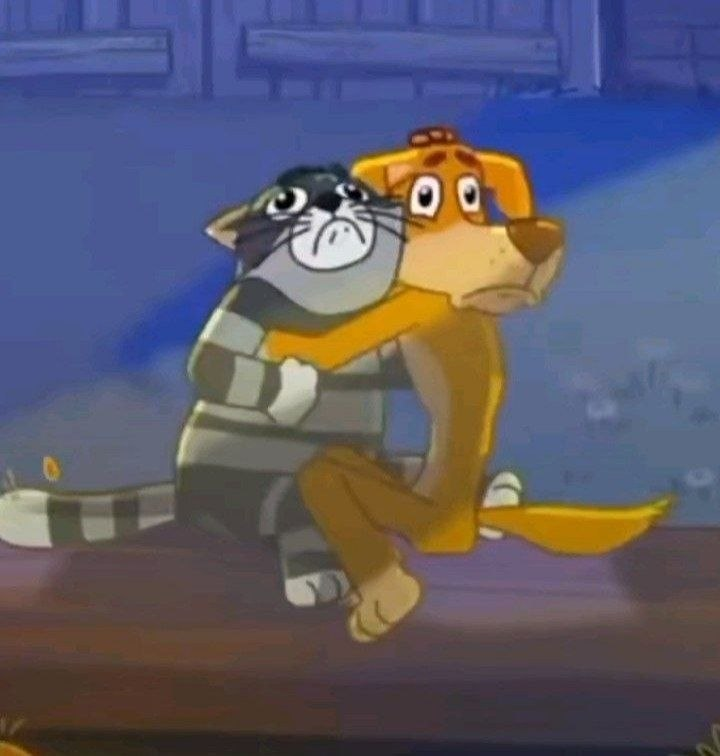
\includegraphics[width=0.7\linewidth]{Простоквашино.jpg}
\end{figure}


\end{document}